\documentclass[memoire.tex]{subfiles}
\begin{document}
\section{Notions de dynamique}
\subsection{Introduction}
Jusqu'ici, on s'intéressait au changement du lieu d'annulation d'une fonction $F$. Dans un contexte de dynamique, ça correspond à étudier la façon dont les points d'équilibre changent lorsqu'un paramètre varie, et on "oubliait" en quelque sorte la dynamique dont était originaire la fonction, ce qui invisibilise certaines propriétés de ces équilibres. Reprenons la dynamique de l'exemple \ref{Poutre}, en considérant le premier mode de flambement
\begin{equation*}
    F(\theta,\lambda)=D^2 \theta + (\lambda+n^2\pi^2) \sin\theta =0
\end{equation*}

Intuitivement, on sent bien que si on dépasse la valeur 
critique, alors la poutre va forcément se tordre 
(dans une des 2 directions !) et qu'il est impossible que 
le système reste sur la ligne triviale. On a donc bien 
envie de pouvoir distinguer les "vrais" équilibres, 
physiquement réalistes, et ces équilibres "fantômes" qui 
n'existent que mathématiquement. C'est là que la notion de 
\coldef{stabilité} intervient : les solutions de la branche 
triviale, une fois la valeur critique dépassée, sont 
\coldef{instables}. Cette section est adaptée de \cite{kielhoefer2012bta}\\
On se place dans un contexte dynamique: on suppose que que $F$ apparaît dans une équation du type
\begin{equation*}
    \frac{dx}{dt}=F(x,\lambda)
\end{equation*}
On suppose bien sûr que $X\subseteq Y$ (ou s'y plonge continûment)
\begin{definition}
    Si $V$ est un espace vectoriel, le \coldef{complexifié} $V^{\mathbb{C}}$ de $V$ est donné par 
    \begin{equation*}
        V^{\mathbb{C}}=V\otimes_{\R}\mathbb{C}\cong V\oplus i V=\left\{ v_1+iv_2\big| v_1,v_2\in V\right\}
    \end{equation*}
\end{definition}
Si $X$ est un espace de Banach, on munit habituellement son complexifié de la norme 
\begin{equation*}
    ||x+iy||_{X^\mathbb{C}}= \sup_{\theta\in[0,2\pi]} ||x\cos\theta + y\sin \theta ||
\end{equation*}
On vérifie facilement que cette dernière en fait un espace 
de Banach. Quand on parle du spectre de l'opérateur $D$, on parle en réalité de l'opérateur complexifié 
\begin{equation*}
    D^{\mathbb{C}}: X^{\mathbb{C}}\rightarrow X^{\mathbb{C}}
, x+iy\mapsto Dx +iDy
\end{equation*}
\begin{definition}
    On définit $\sigma(D)$ \coldef{le spectre} de $D$ comme étant l'ensemble des complexes $\lambda$ pour lesquels $D-\lambda I$ n'est pas inversible
\end{definition}

\begin{definition}\label{def-stab}
    $x_0$ est un \coldef{point d'équilibre} pour $\lambda_0$ si $F(x_0,\lambda_0)=0$ et c'est un \coldef{équilibre stable} si le spectre de $D_1 F(x_0,\lambda_0)$ est dans le demi plan complexe gauche et si zéro n'est pas valeur propre de $D_1 F(x_0,\lambda_0)$
\end{definition}

La définition précédente peut paraître bien 
arbitraire, mais il s'avère que dans la plupart 
des problèmes pratiques elle se traduit en une 
"vraie" stabilité dynamique. Préciser les 
conditions dans lesquelles ce principe est correct 
et démontrer les résultats associés alourdirait 
le texte, mais il a été montré dans \cite
{henry1981geometric} qu'il est vérifié pour une 
large classe d'opérateurs (dits "sectoriels"). On se contente pour l'instant de donner une justification intuitive dans un cas simple : supposons $X=\R^n$ et supposons que la dynamique se décrit de la façon suivante: 

\begin{equation*}
    \frac{dx}{dt}=-\nabla V(x,\lambda)=F(x,\lambda).
\end{equation*}
C'est extrêmement courant dans le cadre de problème issus de la physique ($V$ est alors le potentiel). Si par exemple $V:\R^2\rightarrow \R$
alors l'équation ci dessus correspond à étudier la vitesse d'un mobile qu'on aurait "déposé" sur la surface décrite par $V$.
On a alors
\begin{equation*}
    D(-\nabla V)(x_0,\lambda_0)=-\operatorname*{Hess}(V)(x_0,\lambda_0).
\end{equation*}
Pour avoir un équilibre stable, il faut que la courbe soit localement un "bol" i.e que la courbure soit totalement positive, donc que toutes les valeurs propres de la Hessienne soit positives et donc que toutes les valeur propre de $DF$ soit négatives. On peut déjà noter, et ça sera crucial pour la suite, que $DF$ est alors une matrice symétrique, donc toutes ses valeurs propres sont réelles. Nous montrons la validité de ce principe en dimension finie dans la section \ref{eigen-stab}\\

\subsection{Le principe d'échange de stabilité}

Si on se place dans une situation de bifurcation simple alors l'équilibre qui se trouve au croisement $(x_0,\lambda_0)$ des deux courbes n'est pas stable. Le but de cette section est alors de comprendre la stabilité des équilibres qui sont proches, et donc de comprendre comment le spectre, et spécifiquement la valeur propre $0$ se comporte au voisinage de $(x_0,\lambda_0)$.\\



\begin{proposition}\label{courbe-vp}
    Soit $F\in C^2(U\times V,Y)$ une fonction de Fredholm d'indice nul.
    Posons $N=\ker D_1F(x_0,\lambda_0)$
    et $R=\im D_1F(x_0,\lambda_0)$ et 
    supposons que
    \begin{equation}\label{transvers-ker}
        N=\rangle v_0\langle_\R\Rightarrow v_0\notin R.
    \end{equation}
    Il existe alors une courbe de solution $\gamma\in C^1(]-\delta,\delta[,X\times \R)$, $\mu\in C^1(]-\delta,\delta [, \R)$ et $w\in C^1(]-\delta,\delta[,X\cap R)$ tels que $w(0)=0$ et
    \begin{equation*}
        D_1F(\gamma)(v_0+w(s))=\mu(s)(v_0+w(s)).
    \end{equation*}
    On dit que $\mu$ est une courbe de valeurs propres perturbées
\end{proposition}
\begin{preuve}
    Posons
    \begin{equation*}
        G: U\times V\times (R\cap X)\times \R\rightarrow Y, (x,\lambda,w,\mu)\mapsto D_1 F(x,\lambda)(v_0+w)-\mu(v_0+w)
    \end{equation*}
    Notez que $G(x_0,\lambda_0,0,0)=0$ et 
    \begin{align*}
        &D_3 G(x_0,\lambda_0,0,0)=D_1 F(x_0,\lambda_0)\\
        &D_4(x_0,\lambda_0,0,0)=-v_0
    \end{align*}
    L'équation \ref{transvers-ker} permet d'affirmer que
    \begin{equation*}
        D_{(2,3)}G(x_0,\lambda_0,0,0): R\cap X\times \R\rightarrow U
    \end{equation*}
    est un isomorphisme, le théorème des fonctions implicites nous donne alors des fonctions $w:U_1\times V_1\rightarrow R\cap X$, $\mu: U_1\times V_1\rightarrow \R$ telles que $x_0\in U_1\subseteq U$ $\lambda_0\in V_1\subseteq V$,  $w(x_0,\lambda_0)=0$, $\mu(x_0,\lambda_0)=0$ et 
    \begin{equation*}
        \forall (x,\lambda)\in U_1\times V_1,G(x,\lambda,w(x,\lambda),\mu(x,\lambda))=0
    \end{equation*}
    qui à réduire $\delta$, on peut supposer 
    $\gamma(]-\delta,\delta[)\subseteq U_1\times V_1$, et
    $\mu\circ \gamma$, $w\circ\gamma$ répondent à la question.
\end{preuve}
Il peut être intéressant, pour
bien comprendre ce qu'il se passe, de 
"suivre" les valeurs propres quand le 
paramètre varie.
\begin{exemple}
 Reprenons encore une 
fois la bifurcation trident, $f(x,\lambda)=x^3-\lambda x$, et calculons 
la stabilité des différentes partie du 
diagramme de bifurcation. $\partial_x f
(x,\lambda)=3x^2-\lambda$ et on 
remarque alors que quand $\lambda$ est 
positif, la branche triviale est stable et instable sinon. Ici, la valeur propre traverse simplement $0$
\end{exemple}
Pour mieux comprendre la condition \ref
{transvers-ker}, on donne un exemple 
ou elle n'est pas respectée
\begin{exemple}
    Considérons
    \begin{equation}\label{ex-nilpot}
        F: \R^2\times \R\rightarrow \R^2, (x,y,\lambda)\mapsto (y,\lambda x-x^3)
    \end{equation}
    On a
    \begin{equation*}
        D_1F(0, 0, \lambda) = 
        \begin{pmatrix} 
            0 & 1 \\ \lambda & 0 \end{pmatrix}
    \end{equation*}
    On remarque que le noyau est égal à l'image quand $\lambda=0$. Maintenant, regardons comment le spectre évolue quand $\lambda$ varie: le polynôme caractéristique est donné par $\mu^2-\lambda$. D'une part, quand lambda positif, on pert le caractère $C^1$. Ensuite, lorsqu'il passe par zéro, toutes les valeurs propres deviennent complexes
\end{exemple}
Il est particulièrement enrichissant de regarder le champ de vecteur associé avec la fonction et d'observer comment il se modifie quand on fait varier le (ou les ) paramètre(s) de bifurcation.
\begin{figure}[htbp]
    \centering
    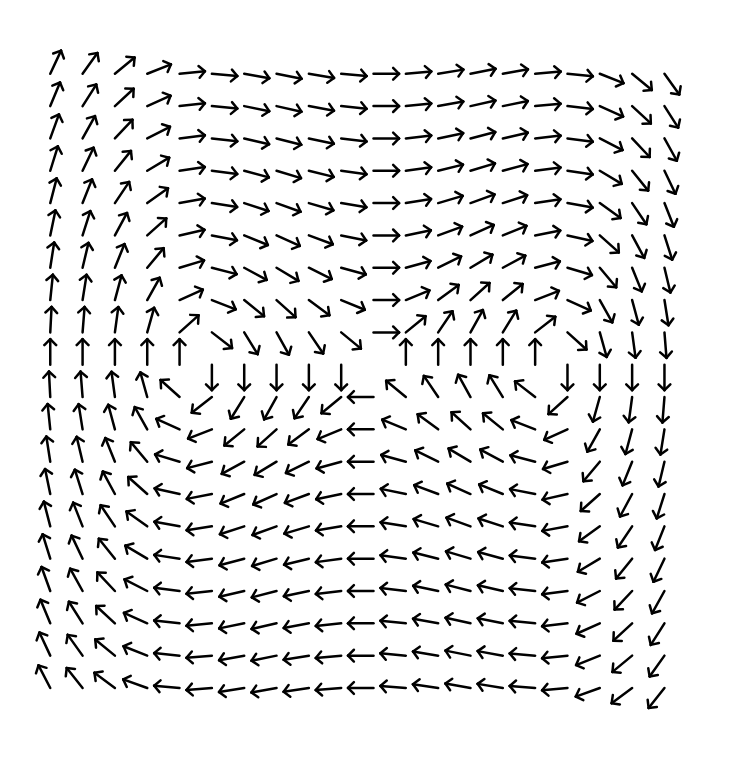
\includegraphics[width=0.32\textwidth]{figures/vectfield_pos.png}
    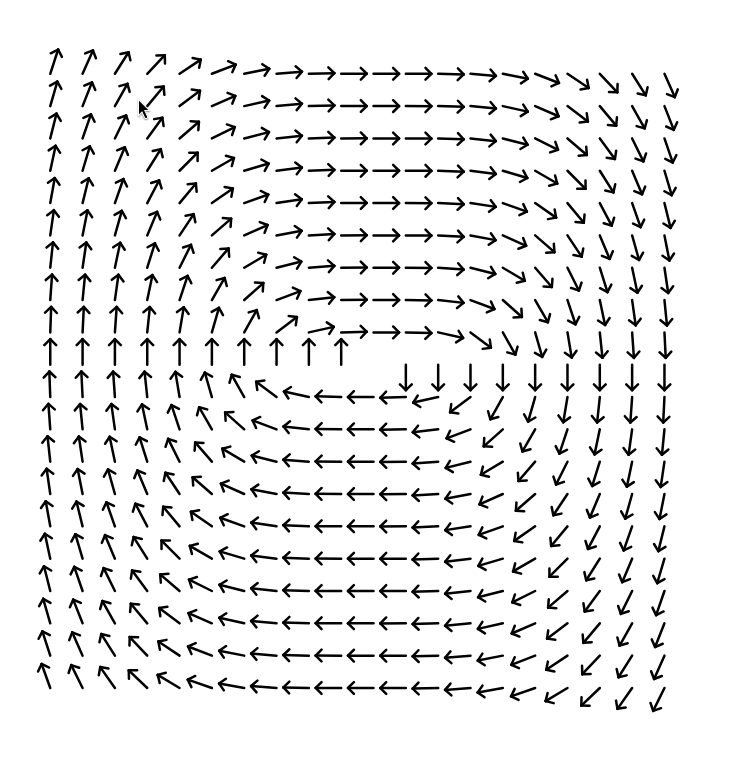
\includegraphics[width=0.32\textwidth]{figures/vectfield_null.png}
    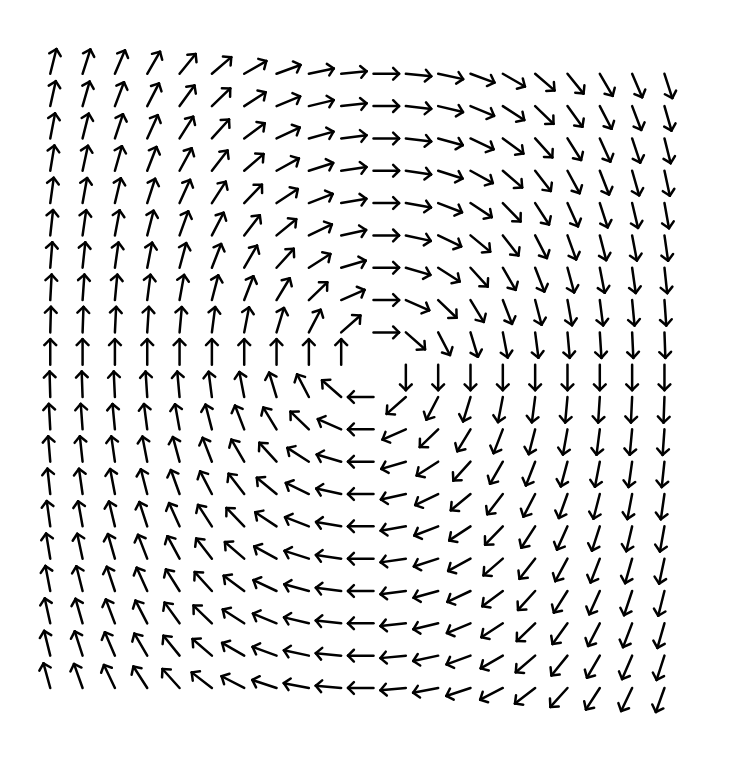
\includegraphics[width=0.32\textwidth]{figures/vectfiled_neg.png}
    \caption{Le champ de vecteur associé à \ref{ex-nilpot} en $\lambda=0.85, 0$ et $-0.85$}
    \label{vectfield_1}
\end{figure}\\
Lorsque $\lambda=0.85$, on a un équilibre (qu'on peut identifier comme instable visuellement) au centre. Et lorsque le $\lambda$ se rapproche de $0$, les deux tourbillons qui se trouvent de part et d'autre fusionnent en un seul.
\begin{remarque}
    En dimension finie la condition de 
    transversalité 
    \eqref{transvers-ker} est équivalente à l'existence d'une base dans laquelle $D_1F(0)$ présente un bloc de jordan nilpotent.
\end{remarque}
La  condition \eqref{transvers-ker}
nous permet d'écrire, avec les notations de la proposition précédente,
\begin{equation*}
    Y=R\oplus N\text{ et donc }
    X=N\oplus (R\cap X)
\end{equation*}
On pose alors $\pi_1: Y\rightarrow N$ et $\pi_2: \pi_1|_{X}$. Du fait que le noyau est de la forme $\rangle v\langle_\R$, le théorème de Hahn-Banach nous assure l'existence d'un élément du dual $v_0^*$ tel que $v_0^{*}(v_0)=1$ et qui est nul sur $\R$. on peut alors écrire $\pi_1$ comme $\pi_1(y)=v_0^{*}(y)v_0$. On peut alors utiliser $\pi_1$ et $\pi_2$ pour faire la réduction de Lyapunov-Schmidt, en effet, on rappelle que la co-image coïncide ici avec la noyau. Rappelons que la fonction $\Phi$ obtenue par cette réduction (c.f 
\eqref{fonctionproj}) nous permet de trouver une courbe de solution, plus précisemment, il existe
\begin{equation*}
    \gamma: ]-\delta,\delta[\rightarrow N\times \R, t\mapsto (\pi_2(t),\lambda(t))
\end{equation*}
telle que $\Phi(\gamma(]-\delta,\delta[))=\left\{0\right\}$.
Maintenant, on se ramène à un problème sur $\R^2$ en posant
\begin{equation*}
    \Psi : U_2\times V_2\rightarrow \R, (y,\lambda)\mapsto v_0^*(\Phi(v_0+yv_0,\lambda))
\end{equation*}
\begin{proposition}
    Avec les notations qui précèdent, on a
    \begin{equation*}
        \partial_s D_1 \Psi(\gamma)(0)=\partial_s \mu(0)
    \end{equation*}
    et si $\partial_s \mu(s)(0)=0$ alors
    \begin{equation*}
        \partial^2_{s}D_1\Psi(\gamma)(0)=\partial^2_s\mu(0)
    \end{equation*}
\end{proposition}

\begin{preuve}
    Soit $\mu(s)$
\end{preuve}

On en tire le résultat suivant
\begin{theobox}{Principe d'échange de stabilité}{}
    feur
\end{theobox}
\subsection{Lien entre spectre et stabilité}\label{eigen-stab}
Ici, on explore plus en détail le lien 
entre le spectre de la jacobienne et 
la stabilité, dans le but de mieux 
justifier la définition \ref
{def-stab}. Dans la suite,$X$ et $Y$ sont des espaces vectoriels de dimension finie. Cette section est basée 
sur [SOURCE].\\
On commence par donner une sens précis à la notion de stabilité. Une façon de faire, attribuée à Lyapunov, est de considérer qu'un équilibre est stable si les solutions aux conditions initiales proches restent proche, d'où la définition suivante
\begin{definition}
    Soit $U\subseteq X$ un ouvert, de $X$, et $x_0\in U$ un équilibre de de $F\in C^1(U,X)$ , i.e $F(x_0)=0$. Dans ce cas, la fonction constante $x_0$  est une solution de
    \begin{equation}\label{eq-dyna}
    \partial_t x= F(x)
    \end{equation} 
    On dit que cet équilibre est  \coldef{stable} si pour tout voisinage $V$ de $x_0$, il existe un voisinage $V_1$ de $x_0$ dans $V$ tel que pour toute solution $f$ telle que $f(0)\in U_1$ est bien définie pour $t>0$ et $f(\R^+)\subseteq  V$. Si de plus, on peut choisir $V_1$ tel que $\lim_{t\to \infty}=x_0$ alors c'est un équilibre asymptotiquement stable
\end{definition}
\begin{exemple}
    Considérons d'abord les équations différentielles du type
    \begin{equation*}
        \partial_t x=Ax
    \end{equation*}
    où $A$ est une matrice réelle et observer le champ de vecteurs en fonction des valeurs propres. La matrice étant réelles, ses valeurs propres $\lambda_1,\lambda_2$ sont soit de la forme $\lambda_1=\alpha+i\beta,\lambda_1=\alpha-i\beta $, $\alpha,\beta$ réels, ou alors toutes les deux réelles. Ci dessous des représentations des champ de vecteurs pour les cas ou elles sont toutes les deux $<0$, de signes opposés et toutes les deux $>0$, respectivement.
    \begin{center}
        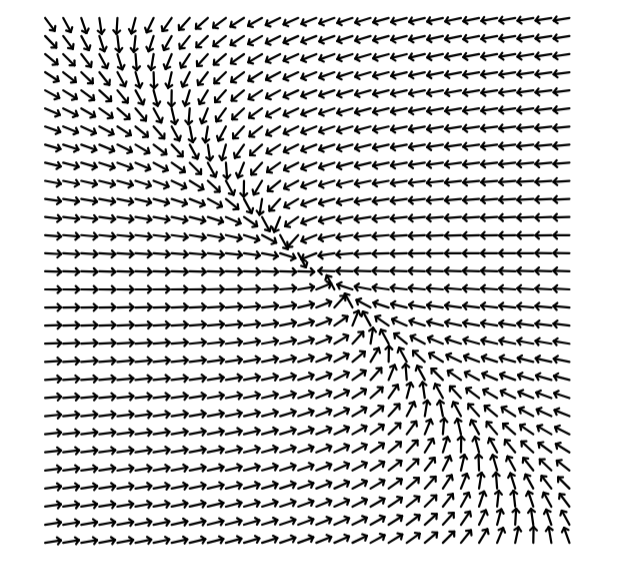
\includegraphics[width=0.32\textwidth]{figures/real_eigen_value_neg.png}
        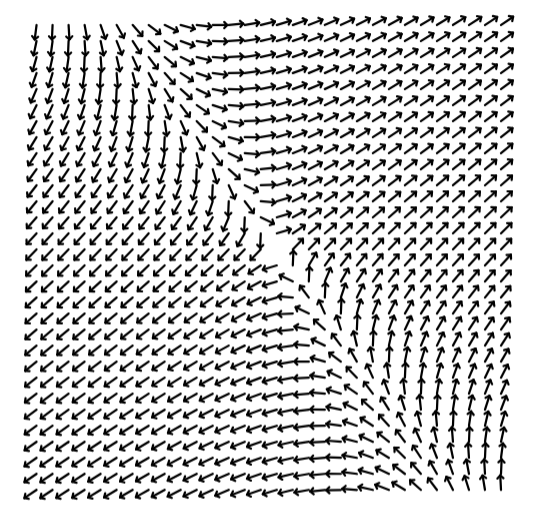
\includegraphics[width=0.32\textwidth]{figures/real_opposite_sign.png}
        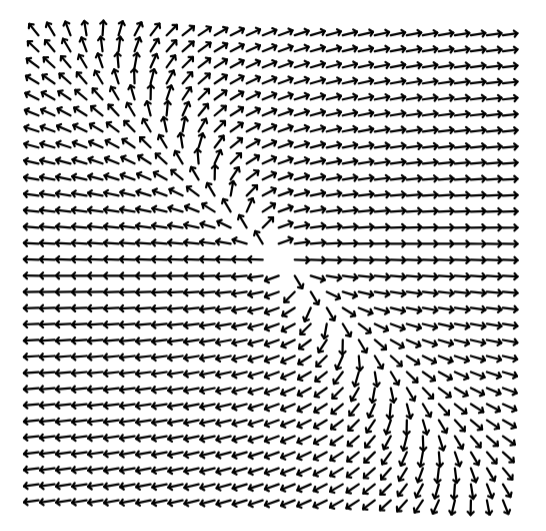
\includegraphics[width=0.32\textwidth]{figures/real_same_sign_plus.png}
    \end{center}
    On a ce qu'on appelle un noeud stable, un noeud instable et un point de selle.
    Maintenant, pour le cas complexe conjugué, on représente les champs de vecteurs dans le cas $\alpha=0$,$\alpha\neq 0$, respectivement
        \begin{center}
        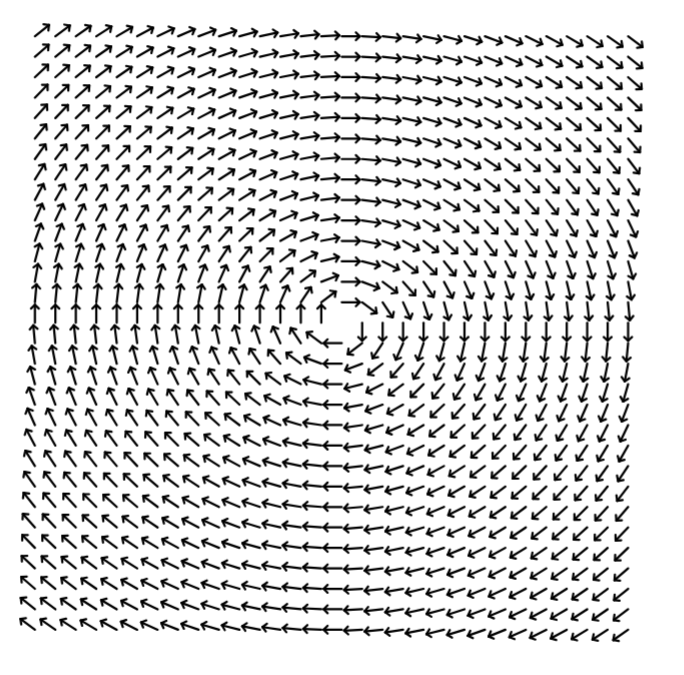
\includegraphics[width=0.32\textwidth]{figures/eigen_image_pur.png}
        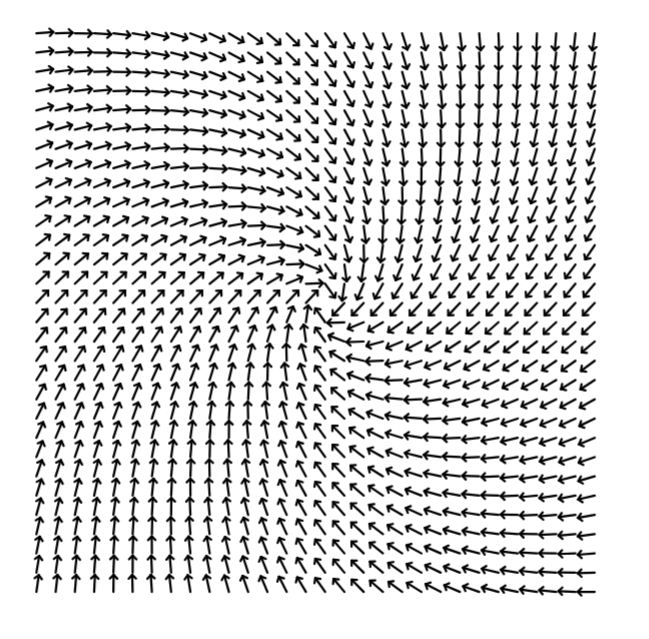
\includegraphics[width=0.32\textwidth]{figures/comep_n_imag_pure.png}
    \end{center}
    Dans le premier cas, les solutions seront des ellipses, et dans le second, des spirales qui vont vers le centre. On peut déjà voir que dans le premier cas, on a la stabilité mais pas la stabilité asymptotique.
\end{exemple}
\begin{definition}
    On dit qu'un équilibre $x_0$ est 
    \coldef{hyperbolique} si aucune de ses valeurs propres n'a de partie réelle nulle
\end{definition}
Notez que c'est une propriété "générique"
\begin{theorem}
    Soit $U\subseteq X$ un ouvert et $F\in C^1(U,X)$. Supposons que $x_0\in U$  soit un équilibre stable de $\partial_t x=F(x)$. Alors $DF(x_0)$ n'a pas de valeur propres ayant une partie réelle positive
\end{theorem}
\begin{preuve}
    On peut bien sûr supposer $x_0=0$. Supposons alors que $DF(0)$ a une valeur propre dont la partie réelle est positive, et on montre que c'est un équilibre instable. Grâce à la forme de canonique de Jordan réelle, on trouve deux sous espaces vectoriels $X_0,X_1$ tels que $X=X_0\oplus X_1$ et que les valeurs propres de $A=DF(0)|_{X_0}$ sont $>0$ et  celles de $B=DF(0)|_{X_1}$ sont $\leq 0$ via le lemme [LEMME]
    \todo{Terminer preuve}
\end{preuve}





\newpage
\subsection{La bifurcation de Hopf}
On comprend, avec ce qui précède que l'apparition de nouvelle branche stables depuis $(x_0,\lambda_0)$ peut s'expliquer par le fait que la branche principale devient instable et cette perte de stabilité s'explique par le fait qu'une valeur propre réelle simple de $D_1F(0,\lambda)$ quitte la partie gauche du plan complexe pour aller dans celle de droite, en passant par zéro "assez vite". Maintenant,  on s'intéresse à une paire de valeur propre complexes  conjuguées entre elle quittant la partie gauche du plan complexe quand $\lambda$ atteint une valeur critique $\lambda_0$. Et on montrera que dans ce cas, même si zéro n'est pas valeur propre de $D_1 F(0,\lambda_0)$, des nouvelles solutions périodiques peuvent apparaître (mais bien sûr, pas de nouveaux équilibres vu le théorème des fonctions implicites).

\subsection{Bifurcations d'attracteurs}
\newpage
\end{document}